\documentclass[11pt]{article}

\usepackage[margin=0.82in]{geometry}
\usepackage{amsmath}
\usepackage{booktabs}
\usepackage{longtable}
\usepackage{microtype}
\usepackage{xcolor}
\usepackage{xurl}
\usepackage[hidelinks]{hyperref}
\usepackage{placeins}
\usepackage{pgfplots}
\usepgfplotslibrary{groupplots}
\pgfplotsset{compat=1.18}

\setlength{\parindent}{0pt}
\setlength{\parskip}{0.55em}
\definecolor{stressred}{RGB}{184,48,62}
\definecolor{debtblue}{RGB}{48,105,152}
\definecolor{taxgold}{RGB}{185,124,24}

\title{What a Treasury Confidence Shock Would Mean for the Middle Class\\
\large A Fiscal Escape Hatch and a Model-Solved Monetary Endgame}
\author{U.S. Fiscal Dynamics Simulator, version 0.2}
\date{August 23, 2026}

\begin{document}
\maketitle

\begin{abstract}
This note imposes a Treasury confidence shock in late 2026: new federal borrowing costs rise
by 500 basis points, a modest recession occurs, and primary deficits remain on CBO's path.
An immediate fiscal escape hatch would require a 5.99-percent-of-GDP primary-balance
improvement.  Assigned entirely to wages, its static equivalent is a 14.25 percentage-point
surcharge---about \$950 per month for an \$80,000 worker.  If elected officials instead pass
the buck for a decade, debt reaches 172 percent of GDP and modeled interest reaches 14.3
percent of GDP by 2036.  This note then makes the monetary endgame an actual model experiment,
not a historical analogy.  Merely removing the 500-basis-point premium in 2036 does not
stabilize debt: it still reaches 228 percent of GDP ten years later.  A five-year inflation
burst also fails because debt resumes rising after the burst.  With fiscal policy still
unchanged as a share of GDP, the inverse solver finds closure only when the rate backstop is
paired with a full decade of elevated inflation: about 5.38 percent annual inflation, a 69.0
percent total price-level increase and 38.6 percent more price-level growth than baseline.
New Treasury financing averages 3.23 percent, or about -2.04 percent after inflation.  Under
one explicit household-incidence rule---an \$80,000 wage follows baseline prices but not the
additional closure inflation---real purchasing power falls by about \$22,300 per year, or
\$1,858 per month, by 2046.  These are conditional model results and an explicit distribution
rule, not forecasts of Federal Reserve, Congressional, investor, or wage-setting behavior.
\end{abstract}

\section{The answer in one sentence}

If Congress keeps passing the buck after the confidence shock, this paper's selected endgame
is not foreign conquest or a missed coupon: the Federal Reserve backstops Treasury financing,
inflation runs at about 5.38 percent for a decade while new Treasury rates average 3.23
percent, and workers and savers whose nominal incomes or assets fail to rise 38.6 percent
above baseline absorb the debt adjustment through lost purchasing power.

That is the refusal-to-adjust loss allocation selected for this note: \textbf{workers and
holders of nominal claims pay through negative real financing}.  The earlier wage-tax
calculation remains as the explicit fiscal escape hatch.  Neither branch is presented as the
policy authorities' most likely choice.

The parable in Peter and Andrew Schiff's \emph{How an Economy Grows and Why It Crashes}
ends with foreigners acquiring claims on domestic wealth \cite{schiff}.  That is a parable,
not evidence produced by this model.  The simulator does not track creditor nationality,
trade, foreign direct investment, or ownership of U.S. assets.  It can instead quantify a
specific domestic loss allocation: nominal Treasury obligations are paid, but their real
financing cost is held below inflation and unindexed household claims lose purchasing power.

\section{How soon could this become a household problem?}

The simulator has no countdown clock and estimates no crisis date.  CBO likewise states
that the exact point at which a U.S. fiscal crisis might occur is unknown
\cite{cboCrisis}.  A confidence change could precede a particular debt ratio, follow it, or
never take the form imposed here.  What the model can show is the difference between the
\emph{market timing} and the \emph{budget timing}: mortgage rates, bond prices, and financial
conditions can react when investors reprice Treasury risk, while Treasury's own cash
interest bill reacts more slowly as outstanding securities mature.

To avoid implying a twenty-year grace period, this experiment begins in \textbf{2026Q4},
the first modeled quarter after this note's August 2026 date.  Opening debt held by the
public is \$32.216 trillion, or 99.22 percent of GDP.  The date is an explicit stress-test
choice, not a claim that a confidence break began or will begin then.

\subsection*{What the 2026 evidence does and does not show}

There are legitimate warning signs.  Treasury's August 2026 advisory committee reported a
10-year yield near 4.6 percent and a two-year yield near 4.2 percent, with the projected
funding gap widening in fiscal years 2027 and 2028 \cite{tbacAug2026}.  Treasury is actively
using liquidity-support buybacks and planned up to \$38 billion of off-the-run security
purchases in the August--October quarter, in addition to cash-management buybacks
\cite{treasuryRefunding}.  GAO concludes that the deteriorating fiscal outlook creates risks
that could reduce demand and raise borrowing costs \cite{gaoDebt}.  Federal Reserve research
also emphasizes that higher far-forward Treasury rates raise long-term credit costs for
households and businesses \cite{fedForward}.

But those facts are not evidence that the Treasury market has already broken.  The same
August advisory report said that Treasury remained adequately funded for the rest of fiscal
2026, and GAO reported that investor demand remained sufficient to finance borrowing.
Yields can reflect expected monetary policy, inflation uncertainty, the supply of debt,
global capital demand, term premiums, and fiscal concerns simultaneously.  Liquidity-support
buybacks are part of an established debt-management program, not proof of insolvency.

The restrained conclusion is: \textbf{2026 contains warning signals and a costlier financing
environment, not a demonstrated fiscal-confidence break}.  The 500-basis-point shock below
is a severe counterfactual beginning now, not a claim that such a premium is already present.

\section{The stress scenario}

The experiment keeps the existing Treasury cohort engine and changes only the following
paths:

\begin{center}
\begin{tabular}{p{0.25\textwidth}p{0.65\textwidth}}
\toprule
Input & Assumption \\
\midrule
Start and horizon & 2026Q4 through 2036Q3, 40 quarters. \\
New-issuance premium & +500 basis points on new bills, notes, bonds, and TIPS real yields.
FRNs reset from the shocked bill rate. \\
Existing fixed debt & Coupons remain unchanged until maturity. \\
Real growth & -2 percent annualized for four quarters, zero for the next four, then the CBO
baseline without catch-up. \\
Primary deficit & CBO nominal baseline until the wage-tax closure is applied. \\
Inflation & CBO baseline; no extraordinary inflation. \\
Default/repression & None.  Every modeled Treasury obligation is honored at face value. \\
\bottomrule
\end{tabular}
\end{center}

The shock is not applied to the coarse ``other public debt'' category because that category
has no defensible maturity or issuance representation.  The model also assumes that every
auction clears at the imposed rate.  It does not simulate failed auctions, bid--ask spreads,
dealer balance sheets, collateral haircuts, or Federal Reserve intervention.

Each quarter, the engine indexes TIPS, resets FRNs, accrues the inherited coupons, matures
the securities due, refinances their principal, and issues new debt for primary deficits and
cash interest.  The federal interest burden therefore rises through actual modeled rollover,
not through an instantaneous repricing of the entire stock.

\section{The first decade if fiscal policy does nothing}

\begin{center}
\begin{tabular}{lrrrrr}
\toprule
Date & Effective rate & Interest/GDP & Deficit/GDP & Debt/GDP & Repriced \\
\midrule
2026Q4 & 4.61\% & 3.49\% & 5.89\% & 100.63\% & 27.3\% \\
2027Q4 & 5.46\% & 5.72\% & 8.35\% & 107.66\% & 41.6\% \\
2029Q4 & 6.64\% & 7.75\% & 9.96\% & 118.90\% & 61.6\% \\
2031Q4 & 7.38\% & 9.55\% & 11.60\% & 131.20\% & 73.9\% \\
2033Q4 & 8.11\% & 11.78\% & 14.04\% & 146.73\% & 87.4\% \\
2036Q3 & 8.40\% & 14.33\% & 16.50\% & 172.09\% & 92.4\% \\
\bottomrule
\end{tabular}
\end{center}

The effective marketable rate excludes TIPS inflation compensation.  Modeled interest/GDP
includes marketable coupon accruals, TIPS compensation, maturity-floor costs, and the coarse
interest estimate on other public debt.  Modeled deficit/GDP is the primary deficit plus
that modeled interest measure, not CBO's unified deficit definition.

By 2036, the stress path has accumulated \$20.637 trillion more modeled interest than the
unchanged baseline.  Debt/GDP is 172.09 percent instead of 119.13 percent.  The result is not
a prediction of 2036.  It is the path obtained by prohibiting fiscal, monetary, issuance,
and market responses for ten years.

\begin{figure}[ht]
\centering
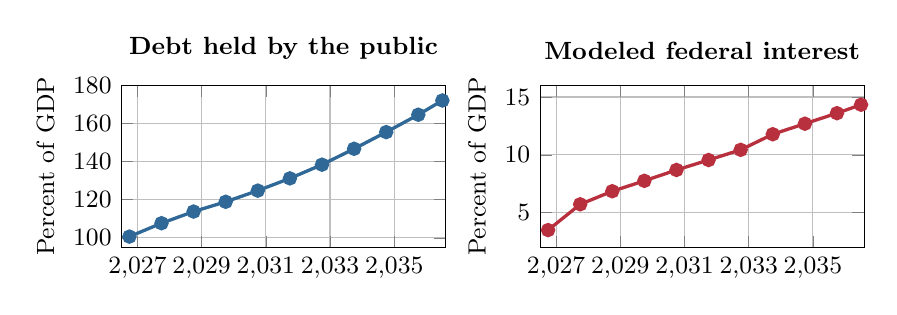
\begin{tikzpicture}
\begin{groupplot}[
  group style={group size=2 by 1, horizontal sep=1.2cm},
  width=0.47\textwidth,
  height=0.30\textwidth,
  xmin=2026.5, xmax=2036.6,
  xtick={2027,2029,2031,2033,2035},
  grid=major,
  tick label style={font=\small},
  label style={font=\small},
  title style={font=\small\bfseries}
]
\nextgroupplot[
  title={Debt held by the public},
  ylabel={Percent of GDP},
  ymin=95, ymax=180
]
\addplot[debtblue, very thick, mark=*] coordinates {
  (2026.75,100.63) (2027.75,107.66) (2028.75,113.78) (2029.75,118.90)
  (2030.75,124.77) (2031.75,131.20) (2032.75,138.39) (2033.75,146.73)
  (2034.75,155.49) (2035.75,164.61) (2036.50,172.09)
};
\nextgroupplot[
  title={Modeled federal interest},
  ylabel={Percent of GDP},
  ymin=2, ymax=16
]
\addplot[stressred, very thick, mark=*] coordinates {
  (2026.75,3.49) (2027.75,5.72) (2028.75,6.85) (2029.75,7.75)
  (2030.75,8.69) (2031.75,9.55) (2032.75,10.43) (2033.75,11.78)
  (2034.75,12.69) (2035.75,13.60) (2036.50,14.33)
};
\end{groupplot}
\end{tikzpicture}
\caption{The imposed +500 basis-point premium with no fiscal response.  Existing fixed-rate
coupons do not jump; the burden builds through refinancing and additional borrowing.}
\end{figure}

\section{Passing the buck: every auction clears through 2056}

Now remove the ten-year expiration date from the premium and remove the fiscal response.
From 2026Q4 through the final supported quarter, Congress leaves CBO's primary-deficit path
unchanged.  Treasury issues whatever the cohort engine requires to pay cash interest and
finance the primary deficit, and it replaces every maturing security with a new one.  The
+500 basis-point premium remains on every new bill, note, bond, and TIPS issue.  The same
two-year recession occurs at the beginning, after which real growth returns to the baseline
rate without recovering the lost level.

This is the paper's literal ``pass the buck'' scenario.  It contains no late tax increase,
spending cut, inflation surprise, default, or yield relief.  It is run through 2056Q3 because
that is the last quarter supported by CBO's February 2026 long-term projection data
\cite{cboLongTerm}.  Calling the policy ``indefinite'' means that it persists to the edge of
the model's evidence; the simulator does not manufacture a post-2056 economy.

\begin{center}
\begin{tabular}{lrrrrr}
\toprule
Date & Debt/GDP & Interest/GDP & Deficit/GDP & Net new debt & Gross issuance \\
\midrule
2026Q4 & 100.63\% & 3.49\%  & 5.89\%  & \$0.47T & \$8.13T \\
2036Q3 & 172.09\% & 14.33\% & 16.50\% & \$1.80T & \$18.83T \\
2046Q4 & 316.22\% & 27.69\% & 29.88\% & \$4.77T & \$51.13T \\
2056Q3 & 565.82\% & 50.07\% & 52.37\% & \$11.75T & \$127.85T \\
\bottomrule
\end{tabular}
\end{center}

The two issuance columns are quarterly nominal flows.  ``Net new debt'' is borrowing for
the primary deficit and cash interest.  ``Gross issuance'' also includes replacement of
maturing principal, so it must not be read as new government spending.  Its size matters
because auctions must repeatedly place that volume with investors.

\begin{figure}[ht]
\centering
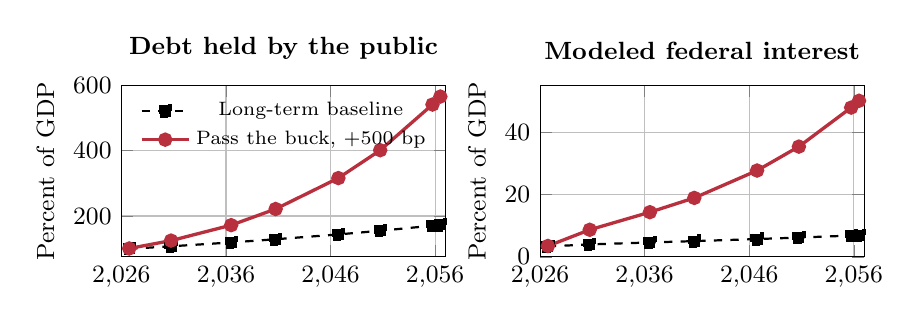
\begin{tikzpicture}
\begin{groupplot}[
  group style={group size=2 by 1, horizontal sep=1.2cm},
  width=0.47\textwidth,
  height=0.31\textwidth,
  xmin=2026, xmax=2057,
  xtick={2026,2036,2046,2056},
  grid=major,
  tick label style={font=\small},
  label style={font=\small},
  title style={font=\small\bfseries},
  legend style={font=\scriptsize, draw=none, fill=none}
]
\nextgroupplot[
  title={Debt held by the public},
  ylabel={Percent of GDP},
  ymin=75, ymax=600,
  legend pos=north west
]
\addplot[black, dashed, thick, mark=square*] coordinates {
  (2026.75,99.62) (2030.75,107.30) (2036.50,119.13) (2040.75,128.90)
  (2046.75,143.68) (2050.75,154.87) (2055.75,170.45) (2056.50,172.77)
};
\addlegendentry{Long-term baseline}
\addplot[stressred, very thick, mark=*] coordinates {
  (2026.75,100.63) (2030.75,124.77) (2036.50,172.09) (2040.75,221.54)
  (2046.75,316.22) (2050.75,401.60) (2055.75,541.49) (2056.50,565.82)
};
\addlegendentry{Pass the buck, +500 bp}
\nextgroupplot[
  title={Modeled federal interest},
  ylabel={Percent of GDP},
  ymin=0, ymax=55
]
\addplot[black, dashed, thick, mark=square*] coordinates {
  (2026.75,3.34) (2030.75,3.99) (2036.50,4.62) (2040.75,5.05)
  (2046.75,5.71) (2050.75,6.19) (2055.75,6.83) (2056.50,6.93)
};
\addplot[stressred, very thick, mark=*] coordinates {
  (2026.75,3.49) (2030.75,8.69) (2036.50,14.33) (2040.75,18.91)
  (2046.75,27.69) (2050.75,35.37) (2055.75,47.89) (2056.50,50.07)
};
\end{groupplot}
\end{tikzpicture}
\caption{Continuous borrowing does not stabilize the stress path.  The simulator keeps
auctions clearing at the imposed yields, so the accounting continues while interest grows
faster than the economy.}
\end{figure}

By 2056Q3, nominal debt is \$518.5 trillion against nominal GDP of \$91.6 trillion.
Modeled interest consumes the equivalent of 50.07 percent of annual GDP; the inherited
primary deficit is only 2.30 percent.  Thus almost the entire 52.37-percent total deficit is
interest on prior borrowing.  Cumulative modeled interest from 2026Q4 is \$449.4 trillion,
versus \$98.3 trillion on the unshocked long-term baseline.  Those are nominal dollars added
across three decades, not present-value or today's-dollar costs.

The engine is then asked a narrow one-quarter question: what primary balance in 2056Q3 would
hold the inherited 557.60-percent debt ratio approximately constant?  Its answer is a
\textbf{primary surplus of 30.57 percent of GDP}.  Relative to the 2.30-percent baseline
primary deficit, that is an immediate improvement of 32.88 percent of GDP.  If the earlier
42-percent wage share were carried forward solely as an illustration, the static wage-tax
equivalent would be 78.3 percentage points.  That is not a viable revenue estimate; it is a
warning that delay has pushed this selected tax-only closure outside a plausible economic
range.

\subsection*{What citizens experience while elected officials do nothing}

The model's government can issue in every supplied quarter because the code requires every
auction to clear.  Real markets provide no such guarantee.  Long before the last line of the
table, households would encounter the consequences the simulator leaves outside its
accounting boundary:

\begin{itemize}
\item New homebuyers, movers, small businesses, state and local governments, and borrowers
  refinancing debt would compete against Treasury at rates anchored to a persistently more
  expensive federal benchmark.  Existing fixed-rate borrowers are initially protected;
  new borrowers are not.
\item Banks, pensions, insurers, retirement funds, and bond funds would carry market-value
  losses on older low-coupon securities.  Higher coupons eventually benefit new savers, but
  only because future taxpayers owe those coupons.
\item To the extent that ever larger Treasury auctions draw private saving, they would leave
  less financing for housing and productive private investment.  The simulator does not
  reduce GDP for this crowding-out channel, so its 2056 denominator is optimistic relative
  to a world in which capital formation suffers.
\item Federal programs remain untouched only by assumption.  By 2056 the modeled interest
  claim is more than twenty times the primary deficit.  The paper is not hiding benefit cuts
  in this run; it is showing that continued issuance postpones the allocation decision while
  making the creditor claim grow.
\end{itemize}

This is not a forecast that the market calmly funds debt equal to 566 percent of GDP.  It is
the opposite: the increasingly implausible issuance requirements identify where the model's
exogenous-market assumption becomes decisive.  The simulator can demonstrate the arithmetic
of passing the buck; it cannot determine the earlier date at which investors, voters,
Congress, or the Federal Reserve would refuse to continue it.

\section{What \$518.5 trillion actually means}

The nominal debt number is not the household result.  It is not a bill delivered to families
in 2056, and nominal dollars thirty years apart are not directly comparable.  Nor does
interest simply disappear from the economy: a Treasury payment is income to a bondholder,
pension, bank, mutual fund, foreign investor, or the Federal Reserve.  One party's federal
asset is the public's liability.

The alarming result is the relationship between financial claims and productive capacity.
At the end of the stress path, the federal government is issuing \$11.75 trillion of
genuinely new debt in one quarter and refinancing enough maturing securities to bring gross
quarterly issuance to \$127.85 trillion.  Interest accruals equal 50.07 percent of annual
GDP.  The simulator obtains that result only because it imposes three conditions that cannot
be presumed to coexist in reality:

\begin{enumerate}
\item investors buy every security at the specified rate, regardless of volume;
\item households and businesses continue producing along the imposed GDP path, despite the
  financing burden; and
\item taxes, benefits, the price level, and the monetary regime never respond.
\end{enumerate}

The path is therefore \textbf{self-invalidating}.  It does not say that \$518.5 trillion is
acceptable.  It says the unchanged regime would almost certainly have changed before the
model reached that number.  Continuous issuance moves the decision through time; it does not
remove the decision.

\section{Use the model: the selected monetary endgame}

The preceding version of this note leaned too heavily on an external historical narrative.
The simulator can answer a narrower but more useful question itself: after ten years of
passing the buck, can a Treasury rate backstop prevent the spiral, and what price-level path
would be required if fiscal policy still does not adjust?

The new experiment inherits the actual 2036Q3 cohort ledger from the stress run: \$77.062
trillion of debt against \$44.781 trillion of nominal GDP, or 172.09 percent.  Expensive debt
issued during the first decade keeps its coupon and maturity.  Beginning in 2036Q4, the
backstop returns rates on new bills, notes, bonds, and TIPS to their CBO baseline paths.  It
does not refinance the entire stock at once.  Primary deficits remain constant as a share of
the scenario's inflated GDP, so surprise inflation does not quietly create a fiscal
adjustment by freezing nominal spending.

The closure target is the standard v0.2 definition: debt/GDP in 2046Q3 must be no higher than
the inherited 172.09 percent, and the ratio may rise by no more than 0.1 percentage point over
the final four quarters.

\begin{center}
\begin{tabular}{p{0.35\textwidth}rrr}
\toprule
2036Q4--2046Q3 policy & Debt/GDP & Interest/GDP & Final-year change \\
\midrule
Continue the +500 bp premium & 311.51\% & 27.26\% & +18.05 points \\
End the premium; baseline inflation & 227.57\% & 9.70\% & +3.78 points \\
End premium; five-year inflation burst & \multicolumn{3}{c}{No closure solution within the
500\% extra price-level bound} \\
End premium; ten-year solved inflation & 172.09\% & 7.93\% & -1.63 points \\
\bottomrule
\end{tabular}
\end{center}

The backstop alone matters enormously: it saves \$54.25 trillion of modeled interest relative
to continued stress over the second decade.  But it does not close the system.  Debt still
rises to 228 percent of GDP because the inherited high-coupon stock and baseline primary
deficits continue adding debt.

The failure of the five-year inflation burst is more revealing.  Even at the solver's extreme
upper bound---a 500-percent additional price-level increase---the ratio is materially rising
again in the final year.  The huge shock lowers the debt ratio's level, but once inflation
returns to baseline the adverse flow reappears.  A temporary price-level trick cannot
permanently repair an unchanged primary-deficit path.

The model does find a mathematical closure when inflation and the rate backstop both persist
for the full second decade:
\[
\text{additional price-level factor}=1.38637,
\qquad
\bar\pi_{2036:2046}=5.3845\%.
\]
The total price level rises 68.95 percent, compared with 21.87 percent on the baseline price
path.  Equivalently, the closure requires 38.64 percent more cumulative price growth than
baseline.  Nominal debt does not disappear: it rises from \$77.06 trillion to \$154.18
trillion.  Nominal GDP rises to \$89.60 trillion, leaving debt/GDP back at 172.09 percent and
falling over the final year.

\begin{figure}[ht]
\centering
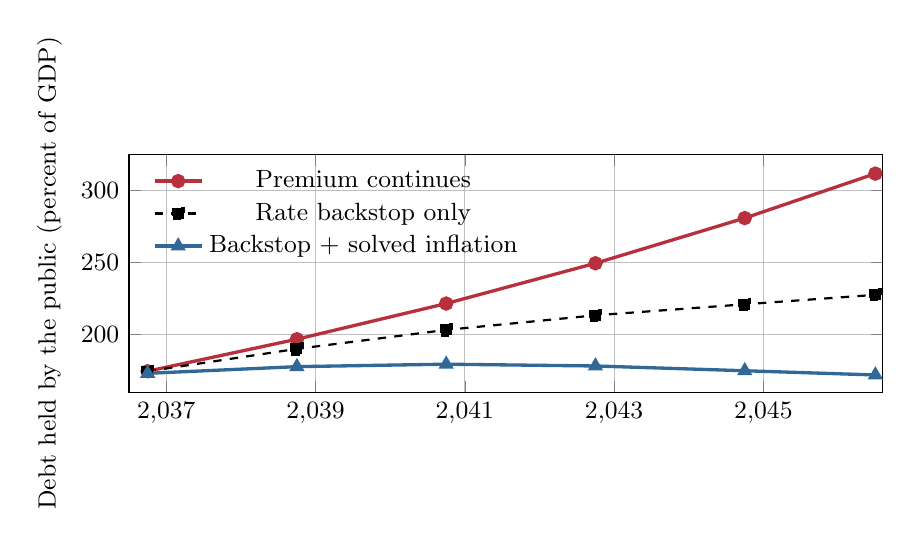
\begin{tikzpicture}
\begin{axis}[
  width=0.92\textwidth,
  height=0.38\textwidth,
  xmin=2036.5, xmax=2046.6,
  xtick={2037,2039,2041,2043,2045},
  ymin=160, ymax=325,
  ylabel={Debt held by the public (percent of GDP)},
  grid=major,
  legend style={font=\small, draw=none, fill=none, at={(0.02,0.98)}, anchor=north west},
  tick label style={font=\small},
  label style={font=\small}
]
\addplot[stressred, very thick, mark=*] coordinates {
  (2036.75,174.69) (2038.75,196.85) (2040.75,221.54)
  (2042.75,249.44) (2044.75,280.73) (2046.50,311.51)
};
\addlegendentry{Premium continues}
\addplot[black, dashed, thick, mark=square*] coordinates {
  (2036.75,174.64) (2038.75,190.16) (2040.75,203.28)
  (2042.75,213.40) (2044.75,221.03) (2046.50,227.57)
};
\addlegendentry{Rate backstop only}
\addplot[debtblue, very thick, mark=triangle*] coordinates {
  (2036.75,173.22) (2038.75,177.85) (2040.75,179.55)
  (2042.75,178.31) (2044.75,175.01) (2046.50,172.09)
};
\addlegendentry{Backstop + solved inflation}
\end{axis}
\end{tikzpicture}
\caption{What the model says happens after the first decade.  Ending the premium slows the
spiral but does not stabilize debt.  Persistent inflationary closure first permits a modest
further rise, then returns the ratio to its inherited level as negative real financing works
through the cohort stock.}
\end{figure}

This is financial repression in the simulator's narrow sense.  Gross principal refinancing
over the decade is \$1{,}024.8 trillion because short instruments can roll repeatedly; that
is turnover, not a trillion-dollar stock existing at one time.  New Treasury issuance
averages 3.23 percent while inflation averages 5.38 percent, an approximate ex-post real
financing rate of -2.04 percent.  TIPS are not treated like nominal bonds: extra indexation
adds \$3.95 trillion of principal compensation.  In an order-dependent accounting bridge,
the nominal-GDP denominator lowers terminal debt/GDP by 63.42 percentage points relative to
the rate-cap-only path, TIPS indexation gives back 5.02 points, and scaling the primary
deficit with scenario GDP gives back another 2.92 points.  The net improvement is 55.49
points.

The hard conclusion is therefore specific.  \textbf{In this model, a central-bank rate
backstop is not enough.  If Congress still refuses a primary adjustment, closure requires a
decade in which inflation persistently outruns Treasury financing rates.}  That is a transfer
from holders of unindexed nominal claims to the federal debtor, not the disappearance of
nominal debt.

\subsection*{What the average household experiences}

The burden would not arrive as a statement reading ``your share of \$518.5 trillion.''  It
would arrive through ordinary prices, paychecks, balance sheets, and public institutions:

\begin{longtable}{p{0.25\textwidth}p{0.65\textwidth}}
\toprule
Transmission & Household consequence \\
\midrule
\endhead
Treasury-rate shock & New mortgages, auto loans, business credit, and state and local
borrowing become more expensive.  Existing fixed-rate mortgages initially retain their
contractual rates. \\
Bond-price decline & Bond funds, pensions, banks, insurers, and retirement portfolios lose
market value on old low-coupon assets.  A household does not need to own Treasury securities
directly to be exposed. \\
Recession and crowding out & Construction and interest-sensitive investment weaken; hiring
and wage growth suffer.  More saving finances federal rollover rather than new homes,
equipment, and productive businesses. \\
Federal Reserve backstop & Cash, wages, pensions, and fixed coupons lose purchasing power if
they adjust more slowly than prices.  Fixed-rate debtors may gain in real terms, while savers
and creditors lose. \\
Weaker dollar & Imported consumer goods and imported inputs become more expensive.  U.S.
households command fewer foreign goods and services for a given amount of work. \\
Reduced federal capacity & Even when every nominal benefit check clears, the government has
less real capacity for defense, infrastructure, disaster response, research, health, and
social insurance without creating still more claims. \\
Distributional conflict & The losses differ across workers, retirees, debtors, creditors,
taxpayers, and benefit recipients.  Political conflict intensifies because every attempted
closure reallocates real income and wealth. \\
\bottomrule
\end{longtable}

For a concrete middle-class translation, this note chooses one incidence rule rather than
writing ``some combination.''  Start with an \$80,000 wage in 2036.  Let it rise with the
baseline price path, but not with the additional closure inflation.  The wage therefore
reaches \$97,495 in 2046, while preserving its original purchasing power under the solved
price path would require \$135,163.  In 2036 dollars, the worker's 2046 wage buys what
\$57,705 bought at the start:

\begin{center}
\begin{tabular}{lr}
\toprule
Selected household consequence in 2046 & Model-linked amount \\
\midrule
Real annual wage purchasing power & \$57,705 \\
Real annual loss relative to baseline & \$22,295 \\
Real monthly loss relative to baseline & \$1,858 \\
Real principal value of a fixed nominal \$100,000 claim & \$59,188 \\
Extra nominal wage growth needed above baseline to avoid the loss & 38.64\% \\
\bottomrule
\end{tabular}
\end{center}

This is a selected wage-setting rule, not a wage forecast.  It makes the incidence explicit:
the worker does not receive an automatic cost-of-living adjustment for the additional
inflation.  If wages did rise the full 38.64 percent above baseline, the loss would move to
employer margins, output prices, employment, or another balance sheet; this simulator cannot
allocate that second-round burden.  The \$100,000 row values principal only.  A bond also pays
coupons, and TIPS receive modeled indexation, so it must not be read as a total-return
calculation for every security.

This is the sense in which the risk can become existential.  The simulator does not show the
physical disappearance of the United States, foreign ownership of every American asset, or
the inevitable end of constitutional government.  It does show a path incompatible with
preserving, all at once, the existing tax burden, promised federal programs, stable money,
market-determined Treasury finance, and the current debt stock's real value.

\begin{quote}
\textbf{The defensible conclusion is that unchecked debt can be an existential risk to the
existing U.S. fiscal--monetary regime and to American global primacy.  This simulator does
not establish that it is an existential risk to the continued existence of the American
nation.}
\end{quote}

That distinction is not semantic.  A country can remain sovereign while its households
become poorer, its currency loses international importance, its government has less room to
act, its politics become more conflictual, and another power gains relative influence.  That
is a national decline scenario even without a missed Treasury coupon or a foreign flag over
Washington.

\section{Evidence hierarchy: model, research, and popular narratives}

Ray Dalio and Peter Schiff are treated symmetrically here.  Neither author's narrative is
peer-reviewed validation of this simulator, a probability estimate, or evidence that the
United States is destined to follow a particular historical sequence.  Schiff supplies a
parable about foreign acquisition of domestic claims.  Dalio supplies an historical
archetype linking debt monetization, internal conflict, reserve currencies, and great-power
competition \cite{schiff,dalioChangingOrder,dalioDebtCycle}.  They are useful sources of
questions, not answers generated by the model.

The model result stands without either author: an imposed loss of cheap financing passes
gradually through the Treasury cohort stock; ending the premium alone fails to stabilize the
debt ratio; and a no-fiscal-adjustment monetary closure requires persistent negative real
Treasury financing.  Those are reproducible conditional calculations.

Peer-reviewed fiscal-limit research provides the more appropriate conceptual comparison.
Davig, Leeper, and Walker define the fiscal limit as the point beyond which taxes cannot
rise enough to finance debt; in their rational-expectations model, fiscal spending or
monetary policy must then adjust, and one possible monetary regime produces inflation that
devalues nominal debt \cite{davigLeeperWalker}.  Their model includes expectations and policy
regimes that this simulator lacks.  It supports treating fiscal and inflationary adjustment
as coherent conditional mechanisms; it does not validate this paper's 5.38-percent number or
its assumed rate cap.

The leap from monetary closure to the end of dollar dominance is even less justified.
Gopinath and Stein's peer-reviewed model emphasizes complementarities among trade invoicing,
global banking, and safe-asset demand that can make a dominant currency persistent and grant
its issuer a financing advantage \cite{gopinathStein}.  The current simulator contains none
of those networks.  It therefore cannot determine whether the dollar loses reserve status,
whether another currency can replace it, whether China gains geopolitical leadership, or on
what timetable.  Dalio's great-power story remains a speculative interpretation outside the
model, not the paper's evidentiary spine.

\section{The fiscal escape hatch: a permanent wage tax}

The model solves for a permanent primary-balance improvement of
\[
\Delta PB = 5.9868\% \text{ of GDP}.
\]
This adjustment begins immediately in 2026Q4.  CBO projects wages and salaries at 42 percent
of GDP from 2026 through 2036 \cite{cbo2026}.  This note imposes the entire adjustment as an
employee-side tax on all wages and salaries, with no cap, deduction, credit, or exemption.
The static surcharge is therefore
\[
\tau_w = \frac{0.059868}{0.42}=0.14254,
\]
or \textbf{14.25 percentage points on every dollar of wages}.

At the opening 2026 GDP level, the tax raises approximately \$1.944 trillion per year.  The
tax scales with the wage base thereafter.  It is additional to existing federal, state, and
local taxes.  For context, ordinary Social Security and Medicare taxes total 15.3 percent
when the standard employee and employer shares are combined, although Social Security has a
wage cap and Medicare does not \cite{irs2026}.  The new surcharge is imposed entirely on the
worker in this scenario.

\begin{center}
\begin{tabular}{rrr}
\toprule
Annual wages & New annual tax & Monthly reduction in take-home pay \\
\midrule
\$50,000  & \$7,127  & \$594 \\
\$80,000  & \$11,403 & \$950 \\
\$120,000 & \$17,105 & \$1,425 \\
\$200,000 & \$28,509 & \$2,376 \\
\bottomrule
\end{tabular}
\end{center}

This is a gross-wage calculation.  A married household with two jobs totaling \$120,000
loses \$1,425 of monthly take-home pay before considering its existing taxes, health
premiums, retirement contributions, mortgage, rent, childcare, college saving, or consumer
debt.  The household must reduce consumption or saving, work more, borrow, or draw down
assets.  The federal spending and benefit path is preserved in nominal terms, so the direct
budget loss falls on workers rather than beneficiaries or Treasury creditors.

The distribution is not neutral.  A flat wage surcharge takes the same percentage from a
teacher, nurse, factory worker, engineer, or executive, but it exempts capital gains,
dividends, rents, and the income of retirees without wages.  Younger and middle-aged working
households therefore bear more of the direct burden than many asset-rich retirees.  The tax
also arrives during the imposed recession, when job security and wage growth would already
be under pressure.

\subsection*{What the wage tax accomplishes inside the model}

The surcharge changes the model's positive primary deficit into a primary surplus of roughly
3.4 to 4.2 percent of GDP in the annual checkpoints.  Interest expense still rises because
the +500 basis-point premium is forced to persist even after the tax is enacted.  The model
continues to run total deficits, but nominal GDP growth and the primary surplus keep the debt
ratio from accelerating.  Debt/GDP ends at 93.67 percent in 2036Q3 and rises only 0.10
percentage point over its final four-quarter span, satisfying the default closure condition.

This is a conservative feature in one direction: a credible fiscal correction might reduce
the risk premium, allowing a smaller tax.  It is optimistic in another: the tax has no effect
on labor supply, avoidance, wages, consumption, investment, or GDP.  Both omissions are
material.

\section{Waiting makes the paycheck loss larger}

If the government leaves the +500 basis-point path unchanged and enacts the wage tax later,
the solver uses the debt ratio inherited on that date and the original 2036Q3 deadline:

\begin{center}
\begin{tabular}{rrrrr}
\toprule
Tax begins & Inherited debt/GDP & Fiscal gap & Wage surcharge & Tax on \$80,000 \\
\midrule
2026Q4 & 99.22\%  & 5.99\% GDP & 14.25\% & \$11,403 \\
2028Q4 & 112.61\% & 6.66\% & 15.85\% & \$12,679 \\
2030Q4 & 123.25\% & 7.39\% & 17.59\% & \$14,075 \\
2032Q4 & 136.44\% & 8.20\% & 19.53\% & \$15,627 \\
2034Q4 & 153.32\% & 9.11\% & 21.69\% & \$17,354 \\
\bottomrule
\end{tabular}
\end{center}

These are shrinking-horizon calculations, not rolling ten-year forecasts.  They answer how
large the permanent tax must become if enactment is delayed but the government still insists
on stabilization by the original endpoint.

\begin{figure}[ht]
\centering
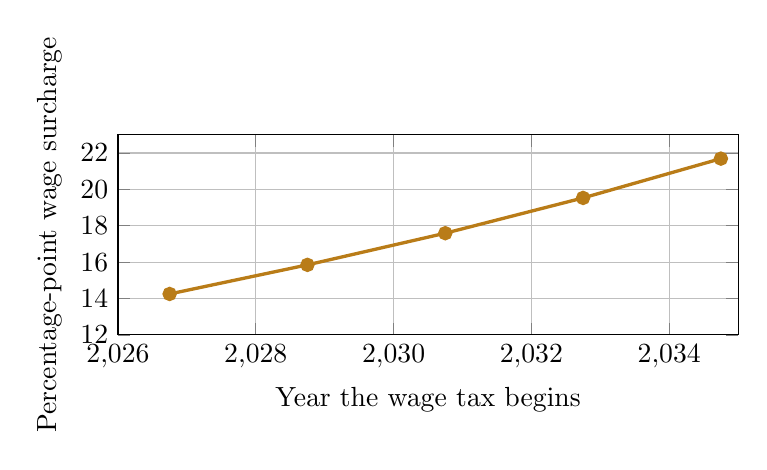
\begin{tikzpicture}
\begin{axis}[
  width=0.78\textwidth,
  height=0.34\textwidth,
  xlabel={Year the wage tax begins},
  ylabel={Percentage-point wage surcharge},
  xmin=2026, xmax=2035,
  ymin=12, ymax=23,
  xtick={2026,2028,2030,2032,2034},
  ytick={12,14,16,18,20,22},
  grid=major,
]
\addplot[taxgold, very thick, mark=*] coordinates {
  (2026.75,14.25) (2028.75,15.85) (2030.75,17.59)
  (2032.75,19.53) (2034.75,21.69)
};
\end{axis}
\end{tikzpicture}
\caption{The static all-wage surcharge required when closure is delayed but the 2036Q3
deadline is retained.}
\end{figure}

\FloatBarrier
\section{What the wage-tax closure would do to middle-class families}

The wage tax is the selected closure, but households would encounter the confidence shock
before the federal interest ledger completed its gradual repricing.

\textbf{Credit and housing.}  Treasury yields are benchmarks for mortgages and other private
borrowing, although private rates would not move one-for-one with the imposed premium
\cite{treasuryPrinciples}.  A household with an existing fixed-rate mortgage keeps that rate.
A renter trying to buy, a family that must move, or a homeowner seeking a new mortgage faces
the new market.  Businesses and landlords facing higher financing costs may reduce
investment or pass costs through where markets permit.

\textbf{Jobs and wages.}  Expensive credit and the imposed recession weaken hiring and
investment.  The 14.25-point wage surcharge then lowers the return to work and reduces
disposable income.  Employers would also face weaker consumer demand as workers cut
spending.  The simulator includes only the imposed growth path, not a second-round recession
from the tax.

\textbf{Retirement accounts and banks.}  Existing fixed-rate bonds retain their contractual
coupons but lose market value when yields rise.  Bond funds, pension portfolios, insurers,
banks, and leveraged investors can therefore experience losses before Treasury's cash
interest cost fully reprices.  The Federal Reserve identifies fixed-rate asset valuation and
Treasury-market liquidity as financial-stability concerns \cite{fedFSR2026}.  The simulator
has face-value debt accounting, not market prices or financial institutions.

\textbf{Public benefits.}  In this deliberately tax-only scenario, baseline Social Security,
Medicare, defense, and other program paths are not cut.  Workers pay to preserve them.  That
does not mean their real quality or political rules would actually remain unchanged; it is
the consequence of selecting one closure mechanism as requested.

\textbf{Saving and consumption.}  A household losing \$950 or \$1,425 each month is likely
to reduce discretionary purchases, retirement saving, education saving, charitable giving,
or housing consumption.  Which margin moves depends on the household.  Aggregated across
workers, those choices become lower demand for businesses and lower private saving or both.

\section{Why 14.25 percent is probably not enough in a real economy}

The calculation divides a 5.99-percent-of-GDP revenue requirement by a wage base equal to
42 percent of GDP.  It assumes the wage base does not shrink when the tax is imposed.  That
is a transparent static translation, not a dynamic revenue estimate.

CBO has examined permanent spending increases of 5 to 10 percent of GDP financed with flat
labor, flat income, or progressive income taxes \cite{cboTaxStudy}.  In those experiments,
tax rates must rise over time to offset behavioral erosion of the tax base, and GDP after a
decade is 3 to 10 percent below the no-policy level depending on the tax design and size.
The exercises are not the same as this confidence shock, but they show why an actual
wage-tax rate would probably need to exceed the static 14.25-point estimate if the risk
premium did not fall.

The result could instead be smaller if the tax restored confidence and reduced Treasury
yields, if productivity rose, or if the government broadened the base beyond wages.  It
could be larger if recessionary deficits widened, market dysfunction raised spreads beyond
500 basis points, the tax reduced labor income sharply, or financial stress required federal
support.  Those are sensitivities, not an invitation to return to an unspecified policy mix:
the policy analyzed here remains a wage tax alone.

\section{What this scenario establishes}

It establishes six conditional results.

First, there is no modeled grace period.  The refinancing mechanism can be shocked in 2026,
and material household consequences appear immediately under the chosen closure even though
Treasury's own interest bill reprices gradually.

Second, a smaller opening debt ratio helps but does not neutralize a persistent 500-basis-
point premium.  With no response, debt reaches 172 percent of GDP and modeled interest
reaches 14 percent of GDP within ten years.

Third, issuing another Treasury security pays the current bill but does not close the system.
If every auction is forced to clear through 2056, interest grows to 50 percent of GDP and the
one-quarter flow-stabilizing primary surplus reaches 30.57 percent of GDP.  The \$518.5
trillion endpoint is evidence that the unchanged-market assumption has become untenable, not
evidence that such a debt stock is acceptable or fundable.

Fourth, the selected monetary endgame is now a model run rather than a Dalio-style assertion.
A rate backstop alone leaves debt at 228 percent of GDP.  A temporary five-year inflation
episode fails the final-year stability condition.  Closure with unchanged fiscal policy
requires the backstop and inflation to persist together for ten years: 5.38 percent average
inflation against 3.23 percent average new Treasury financing.

Fifth, the two explicit loss allocations are severe in different ways.  Avoiding extra
inflation through immediate fiscal closure costs about 14 cents from every wage dollar in the
static tax example, or \$950 per month for an \$80,000 worker.  Refusing that fiscal closure
and selecting monetary closure costs \$1,858 per month in 2036 purchasing power by 2046 under
the paper's explicit no-extra-wage-indexing rule.

Sixth, the most important question is distributional.  Federal debt does not make the
country vanish.  It creates competing claims on future production.  When financing becomes
expensive, closing the arithmetic means deciding whose claim is reduced.  The fiscal-only
branch assigns the direct loss to labor income; the refusal-to-adjust narrative first assigns
real losses to workers and holders of money and fixed-dollar claims whose incomes or assets
do not keep pace with the additional 38.64 percent price-level adjustment.

It does \emph{not} establish that investors will demand a 500-basis-point premium, that the
current Treasury market is broken, that auctions could actually clear along the full 2056
path, that the Federal Reserve can or would impose the assumed rate path, that 5.38-percent
inflation would leave real output and market behavior unchanged, that Congress would select
the tax, that wages would follow the chosen indexing rule, or that Dalio's or Schiff's
narrative predicts the American future.  It is a reproducible stress scenario designed to
turn the model's closure arithmetic into intelligible consequences for citizens.

\section*{Reproducibility}

Run:
\begin{verbatim}
uv run python scripts/run_2026_household_scenario.py
uv run python scripts/run_2036_monetary_backstop_experiment.py
\end{verbatim}
The configurations are stored in
\path{config/scenarios/confidence_shock_2026_household.json} and
\path{config/scenarios/monetary_backstop_2036.json}.  The ten-year paths, delayed-action
results, 2056 pass-the-buck path, monetary-closure diagnostics, and household translation are
stored in CSV files under \path{data/processed/}.  Their prefixes are
\path{confidence_shock_household_2026} and \path{monetary_backstop_2036}.

\begin{thebibliography}{99}

\bibitem{cbo2026}
Congressional Budget Office, \emph{The Budget and Economic Outlook: 2026 to 2036},
February 2026.  \url{https://www.cbo.gov/publication/61882}.

\bibitem{cboLongTerm}
Congressional Budget Office, \emph{The Long-Term Budget Outlook Data: 2026 to 2056},
February 2026.  \url{https://www.cbo.gov/publication/62044}.

\bibitem{cboCrisis}
Congressional Budget Office, \emph{Federal Debt and the Risk of a Fiscal Crisis}, 2010.
\url{https://www.cbo.gov/publication/21625}.

\bibitem{cboTaxStudy}
Congressional Budget Office, \emph{The Economic Effects of Financing a Large and Permanent
Increase in Government Spending}, Working Paper 2021-03.
\url{https://www.cbo.gov/publication/57021}.

\bibitem{tbacAug2026}
U.S. Department of the Treasury, \emph{Report to the Secretary of the Treasury from the
Treasury Borrowing Advisory Committee}, August 2026.
\url{https://home.treasury.gov/news/press-releases/sb0591}.

\bibitem{treasuryRefunding}
U.S. Department of the Treasury, \emph{Quarterly Refunding Statement}, August 2026.
\url{https://home.treasury.gov/news/press-releases/sb0590}.

\bibitem{gaoDebt}
U.S. Government Accountability Office, \emph{Federal Debt Management: Treasury Is Meeting
Borrowing Needs but the Deteriorating Fiscal Outlook Poses Risks}, GAO-26-107529, 2026.
\url{https://files.gao.gov/reports/GAO-26-107529/index.html}.

\bibitem{fedForward}
Board of Governors of the Federal Reserve System, \emph{Why Have Far-Forward Nominal
Treasury Rates Increased So Much in the Past Few Years?}, February 2026.
\url{https://www.federalreserve.gov/econres/notes/feds-notes/why-have-far-forward-nominal-treasury-rates-increased-so-much-in-the-past-few-years-20260212.html}.

\bibitem{treasuryPrinciples}
U.S. Department of the Treasury, \emph{Principles of U.S. Debt Management Policy}, 2024.
\url{https://home.treasury.gov/news/press-releases/jy2460}.

\bibitem{fedFSR2026}
Board of Governors of the Federal Reserve System, \emph{Financial Stability Report}, May
2026.  \url{https://www.federalreserve.gov/publications/files/financial-stability-report-20260508.pdf}.

\bibitem{irs2026}
Internal Revenue Service, \emph{Publication 15 (2026), Employer's Tax Guide}.
\url{https://www.irs.gov/publications/p15}.

\bibitem{davigLeeperWalker}
Troy Davig, Eric M. Leeper, and Todd B. Walker, ``Inflation and the Fiscal Limit,''
\emph{European Economic Review}, vol. 55, no. 1, 2011, pp. 31--47.
\url{https://doi.org/10.1016/j.euroecorev.2010.11.005}.

\bibitem{gopinathStein}
Gita Gopinath and Jeremy C. Stein, ``Banking, Trade, and the Making of a Dominant
Currency,'' \emph{Quarterly Journal of Economics}, vol. 136, no. 2, 2021, pp. 783--830.
\url{https://doi.org/10.1093/qje/qjaa036}.

\bibitem{dalioChangingOrder}
Ray Dalio, \emph{The Changing World Order: The New Paradigm}, January 2022.
\url{https://www.linkedin.com/pulse/changing-world-order-new-paradigm-ray-dalio}.

\bibitem{dalioDebtCycle}
Ray Dalio, \emph{How Countries Go Broke: Introduction \& Chapter One}, January 2025.
\url{https://www.linkedin.com/pulse/how-countries-go-broke-introduction-chapter-one-ray-dalio-3wjae}.

\bibitem{dalioDebtSqueeze}
Ray Dalio, \emph{How Countries Go Broke: Chapter Four \& Chapter Five}, January 2025.
\url{https://www.linkedin.com/pulse/how-countries-go-broke-chapter-four-five-ray-dalio-hqqzc}.

\bibitem{schiff}
Peter D. Schiff and Andrew J. Schiff, \emph{How an Economy Grows and Why It Crashes},
Wiley, 2010.  \url{https://www.wiley-vch.de/en/areas-interest/finance-economics-law/how-an-economy-grows-and-why-it-crashes-978-0-470-52670-5}.

\end{thebibliography}

\end{document}
